% !TEX root = ../thesis_main.tex
\chapter{Results}\label{chap:results}
    As a large part of this work consisted of hardware design and manufacturing, I will split the
    results section into sole hardware results and measurements with that hardware as well as commercially available machines.
\section{Hardware}
    \subsection{Low field NMR}
        \subsubsection{Receive coils}
            Receive circuits provided q-factors of \todo{measure} resulting in resonances about
            $\SI{1}{\kilo\hertz}$ wide. Note that the connection to the NI DAQ introduces additional
            capacities and inductances that cannot be neglected especially in the higher frequency
            range above $\SI{100}{\kilo\hertz}$ where the coil's intrinsic capacities are
            comparatively small.
        \subsubsection{$\mathbf{B_0}$ coils}
            The manufactured $\mathrm{B_0}$ coils show fields (i.e. frequencies) as well as  linewidths in the order of magnitude the
            simulations predicted. Through manufacturing errors, and changes to the coil in long
            term use cases, the linewidths deteriorated. It is important to note that, at currents
            above $\SI{1}{\ampere}$, the $\mathrm{B_0}$ coil heated noiticabely. while the heating
            itself is unproblematic, the resulting exansion of the materials leads to an overall
            longer coil and thus lower fields \ref(fieldSolenoid). To avoid field shifts during
            measurements, the setup should therefore be in thermal equilibrium. This is especially
            relevant when switching fields during measurements using the programmable power supply.
        \subsection{Shims and programmable power supply}
            The three linear shims are adjustable via the programmable power supply and show
            their expected effect. The rotational position of the receive coil is relevant to the
            shims indicating they're working as intended. Using the added shim tool, line widths
            were reduced from $\approx \SI{250}{\hertz}$ to $\approx \SI{30}{\hertz}$ in the case of large samples of $\approx
            $\SI{40}{\milli\litre}. If the initial field was generated by a less homogeneous, more
            asymmetric coil in which no signal was visible without shims, signal was discovered and linewidths went down to
            $\approx \SI{50}{\hertz}$.
            \begin{figure}[h]
                \label{fig:results:lowFieldSpectrometer:shims}
                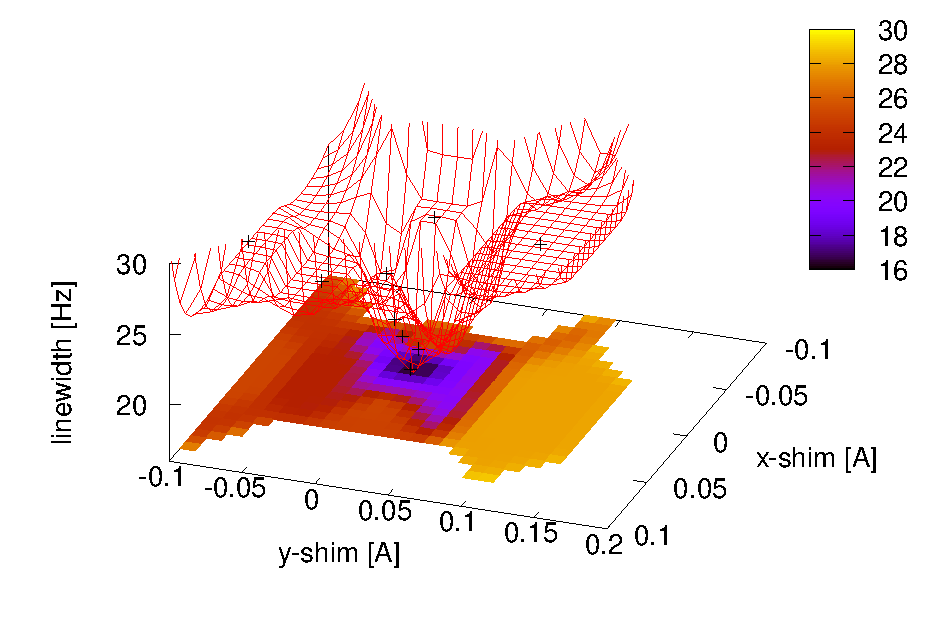
\includegraphics[width=0.9\textwidth]{/figures/experiments/lowFieldSpectrometer/shims/shimXY.eps}
                \caption{Linear shimmung in x- and y-directions. Shimming was done manually: 1H spectra of water were recorded and evaluated as to their linewidth. Later, automatic shimming was implemented (see section \ref{chap:MaterialsAndMethods:lowFieldSpectrometer:shims})}
            \end{figure}
    \subsection{Sabre shuttling system}
        The system designed to transfer a sample between fields works as intended. Fluid losses are
        small and thus acceptable with about \todo{how much} lost within \todo{nn} shuttling cycles at high flow rates of \todo{flow} and long bubbling times of 30 seconds per measurement. The
        bubbling system works well and provides pH2 to the solution in large amounts. 
        \subsubsection{Pressure stability}
        The pressure stability of the vessels has been tested to withstands up to $\SI{50}{\bar}$. Simulations results indicate a factor of safety of $\gamma = 4$ \ref{fig:results:bubblingReactorPressure}.
        \begin{figure}
            \label{fig:results:bubblingReactorPressure}
            \centering
            \includegraphics[width = 0.9\textwidth]{/figures/simulations/15NSabre/bubblingReactorPressure.eps}
            \caption{Wall stress of the low field reactor for bubbling pH2 at \SI{200}{\bar}. As expected, the most vulnerable part is the long side of the cylinder, but wall thickness of \SI{3}{\milli\meter} suffices for a factor of safety of 4 if the setup is operated at \SI{50}{\bar} max.}
        \end{figure}
        
        Chemical resistance is good though resistance to pure pyridine is not given. While there was never
        any problem with the $\SI{}{\milli\Molar}$ pyridine concentrations used in the experiments, a
        neat pyridine batch showed to dissolve the PSU casing.
        \subsubsection{Shuttling reproducibility}
        To ensure that the sample is removed completely from the high field side, spectra in both 'states' of the system were recorded (\ref{fig:results:15N:shuttlingRemoval)}. Integration over both spectra yielded a upper limit of sample remaining inside the high field chamber of which corresponds to an effective polarization reduction of \SI{1}{\percent}.
        \begin{figure}
            \label{fig:results:15N:shuttlingRemoval}
            \centering
            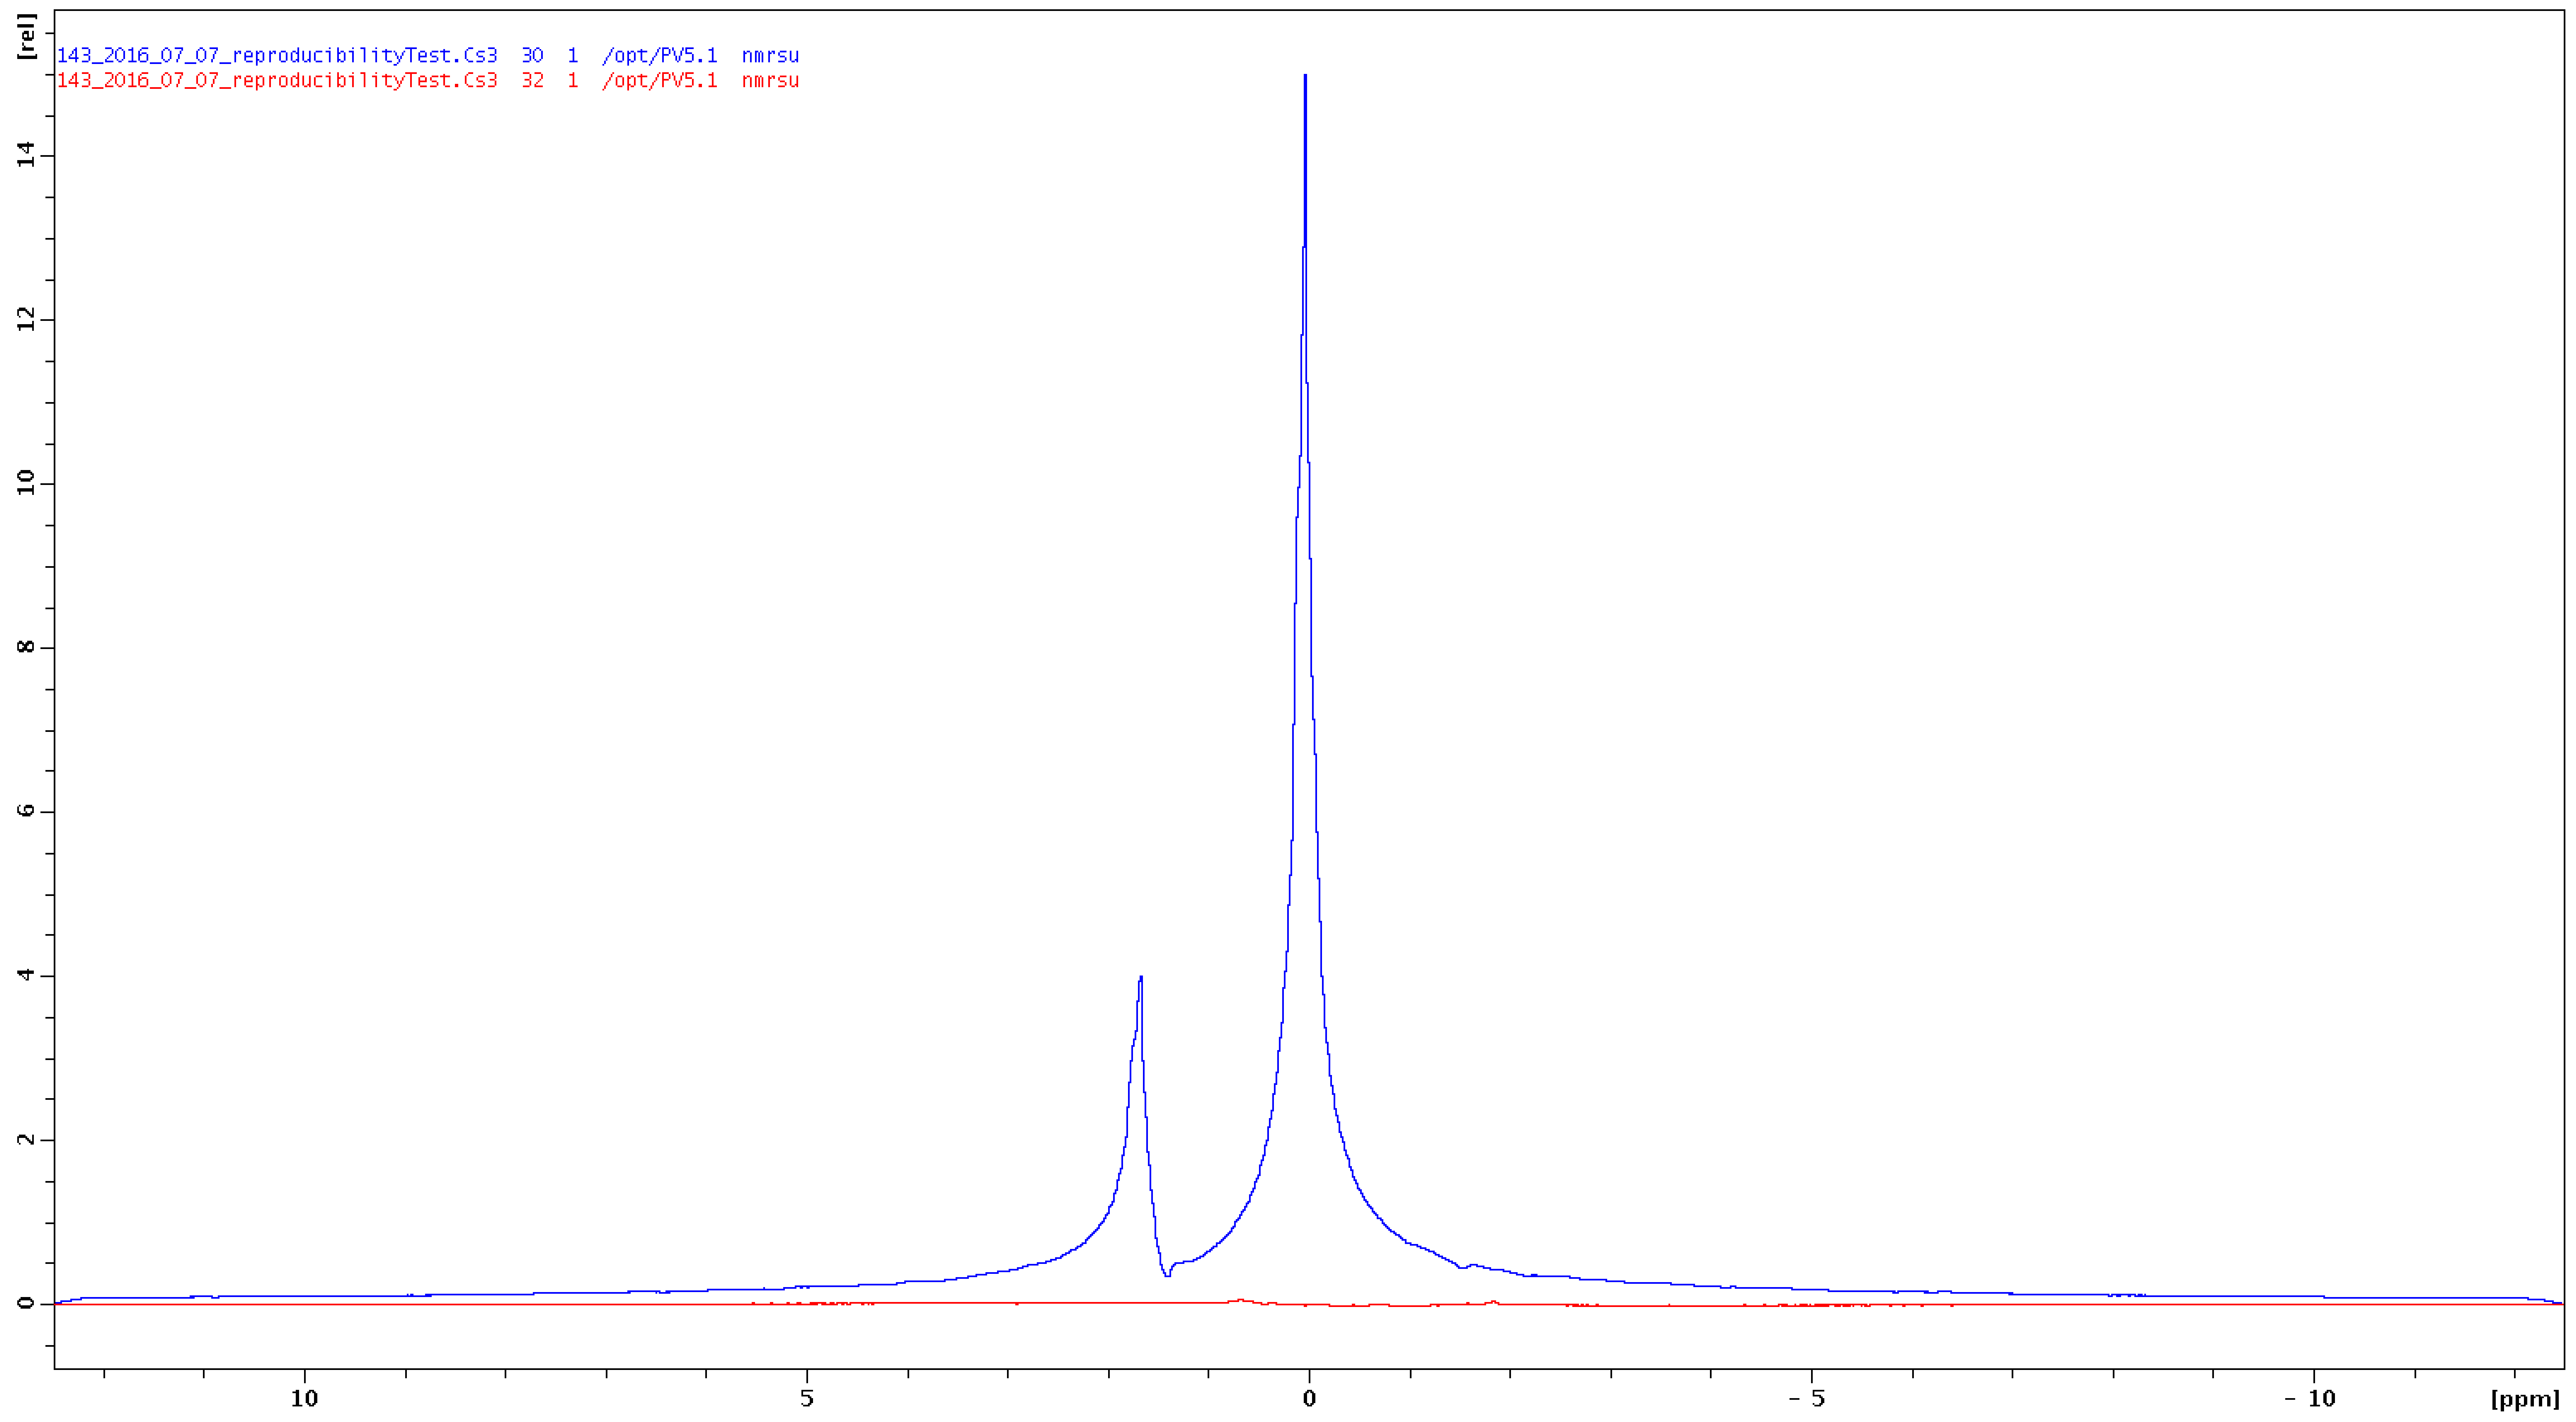
\includegraphics[width=0.9\textwidth]{/figures/experiments/15NSabre/reproducibility/spectraComparisonShuttle.eps}
            \caption{1H spectra of the high field reactor in the filled (blue) and empty (red) state. The filled state delivers a lot more signal as expected while the integration over the empty state spectrum shows a signal reduction of 1000.}
        \end{figure}
        To test the reproducibility of the shuttling system, a hyperpolarized 1H pyridine sample was shuttled back and forth multiple times. The results of the measurement are shown in figure \ref{fig:results:15N:shuttlingReproducibility}. 
        \begin{figure}
            \label{fig:results:15N:shuttlingReproducibility}
            \centering
            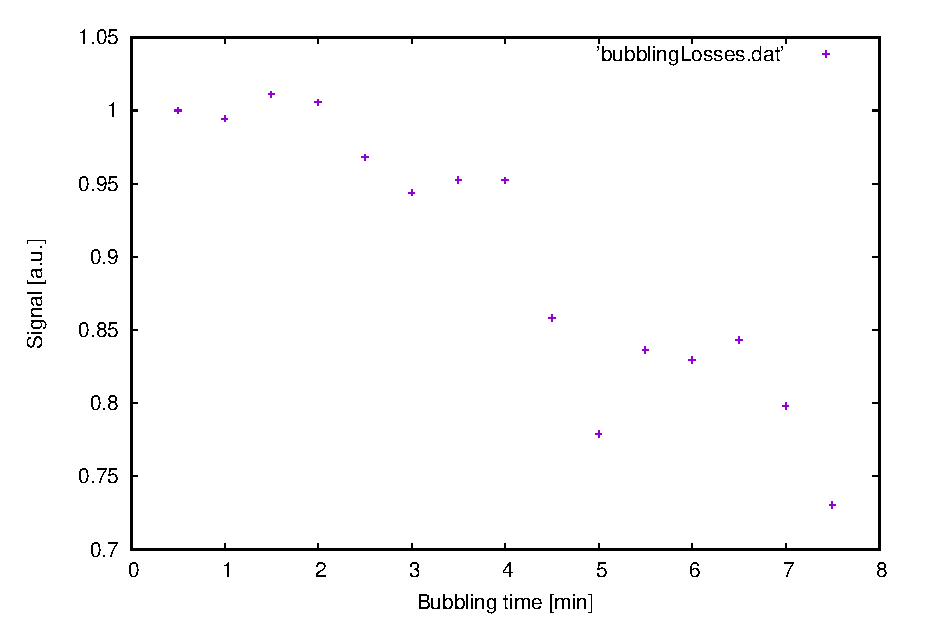
\includegraphics[width=0.9\textwidth]{/figures/experiments/15NSabre/reproducibility/bubblingLosses.eps}
            \caption{Signal intensity during multiple minutes of hydrogen bubbling using a hyperpolarized 1H-pyridine sample. Note that the signal drops to about \SI{70}{\percent} of its initial value after 8 minutes of continuous hydrogen supply. The initial rise of signal during the first two minutes indicates a temperature effect unaccounted for.}
        \end{figure}
    \subsection{Fluxgate readout electronics}
        The readout electronics were designed to feature a wide range of amplifications for all
        three spatial dimensions. A 24 V DC power supply was fitted with a DC-DC-converter to
        provide the $\pm\SI{15}{\volt}$ to power the Fluxgate. Additionally the PCB board was fitted
        with the electronic parts (see \ref{sec:methodsFluxgate}). For testing purposes, a simple program
        using serial in and output to toggle the analog switches was written. All switches were
        successfully tested to work, though three had to be replaced at some point for malfunction.
        Apparently this was due to damage during assembly as the board is now working as expected.
    \subsection{Fluxgate calibration}
    The three spatial channels of the fluxgate sensor needed to be calibrated as to their intrinsic offsets as described in \ref{materialsMethods}. Data for X- and Y-channels are shown in figure \ref{fig:results:fluxgate:xysinus}
        \begin{figure}[h]
            \label{fig:results:fluxgate:ysinus}
            \centering
            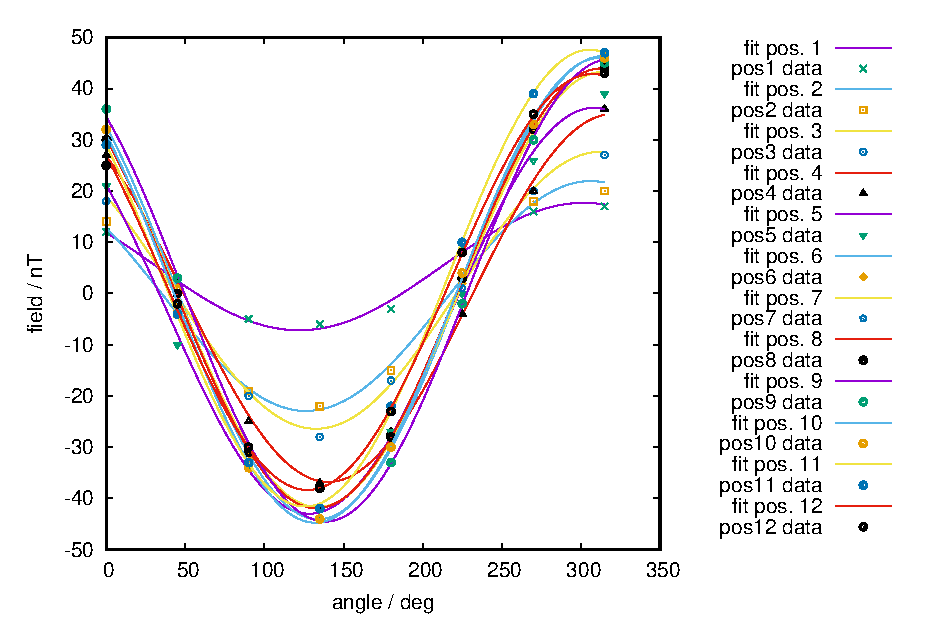
\includegraphics{/home/philipp/Documents/thesis/figures/experiments/fluxgate/xField.eps}
            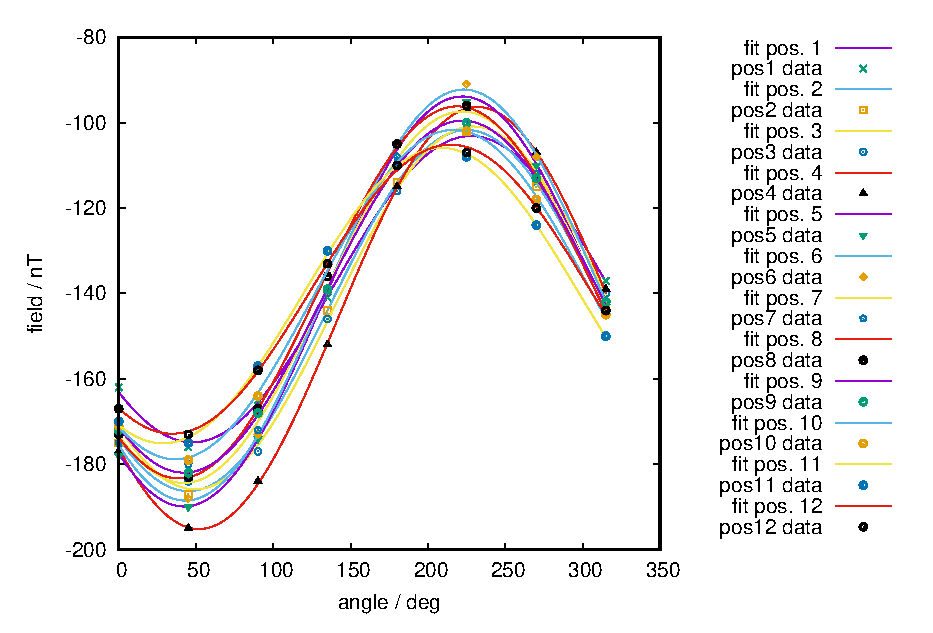
\includegraphics{/home/philipp/Documents/thesis/figures/experiments/fluxgate/yField.eps}
            \caption{Calibration data of X- and Y-channel. Each dataset in the key corresponds to a full rotation at one position in the MuMetal shield. The solid lines correspond to a sine fit to each dataset with phase, amplitude and offset as fitting parameters. Error bars are not displayed for better visibility.}
        \end{figure}
        The fit parameters shown in table \ref{table:results:calibrationFitParams} allow for calibration of X- and Y- channel by calculating the average offset for all Positions.
        \begin{table}
            \centering
            \label{table:results:calibrationFitParams}
            \begin{tabular}{r|cccccccccccc}
                \label{table:results:calibrationFitParams}
                position & 1& 2 & 3 & 4 & 5 & 6\\
                \hline
                amplitude & 22.4 & 27.0 & 35.9 & 39.6 & 45.2 & 42.5\\ 
                offset \\
                phase \\
                \hline
                position & 7 & 8 & 9 & 10 & 11 \\
                \hline
                amplitude & 42.9 & 45.1 & 45.4 & 44.6 & 40.6\\
                offset \\
                phase
            \end{tabular}
        \end{table}
        \begin{figure}[h]
            \label{fig:results:fluxgate:zcal}
            \centering
            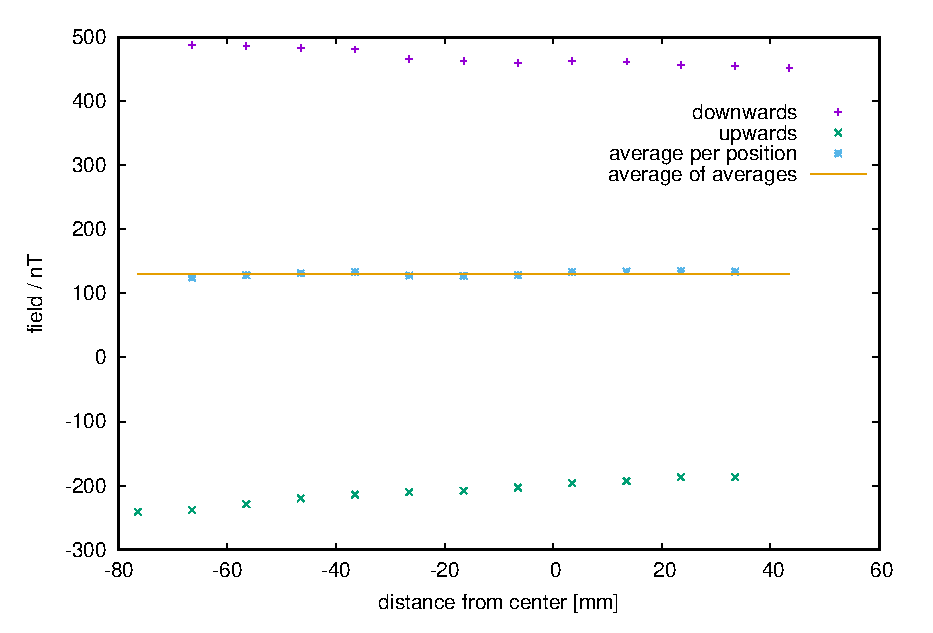
\includegraphics{/home/philipp/Documents/thesis/figures/experiments/fluxgate/zField.eps}
            \caption{Calibration of the Z-channel. Due to spatial limitations, no full rotation in z direction was possible. The two datasets represent one measurement in "upwards" ond one in "downwards" direction. The solid line represents the average of the positional averages of the two directions.}
        \end{figure}
        Using the data for calibration, the measurements of the X- and Y-channels can be used to plot a 2D-section of the field using the phase of the fit as the field direction and the amplitude as its magnitude. Both X- and Y-sensor are shown in figure \ref{fig:results:fluxgate:plotSpatial2d}. The absolute positions are indicated in the figure to enable comparison of the individual results in the same absolute position. The same data is also shown in a 3D plot (fig. \ref{fig:results:fluxgate:plotSpatial3d} to show the field progression inside the mu metal shield.
        \begin{figure}[t]
            \label{fig:results:fluxgate:plotSpatial2d}
            \centering
            %\includegraphics{/home/philipp/Documents/thesis/figures/experiments/fluxgate/spatial2dProjection.eps}
            \includegraphics{/figures/experiments/fluxgate/spatial2dProjection.eps}
        \end{figure}
        \begin{figure}[t]
            \label{fig:results:fluxgate:plotSpatial3d}
            \centering
            %\includegraphics{/home/philipp/Documents/thesis/figures/experiments/fluxgate/spatial2dProjection.eps}
            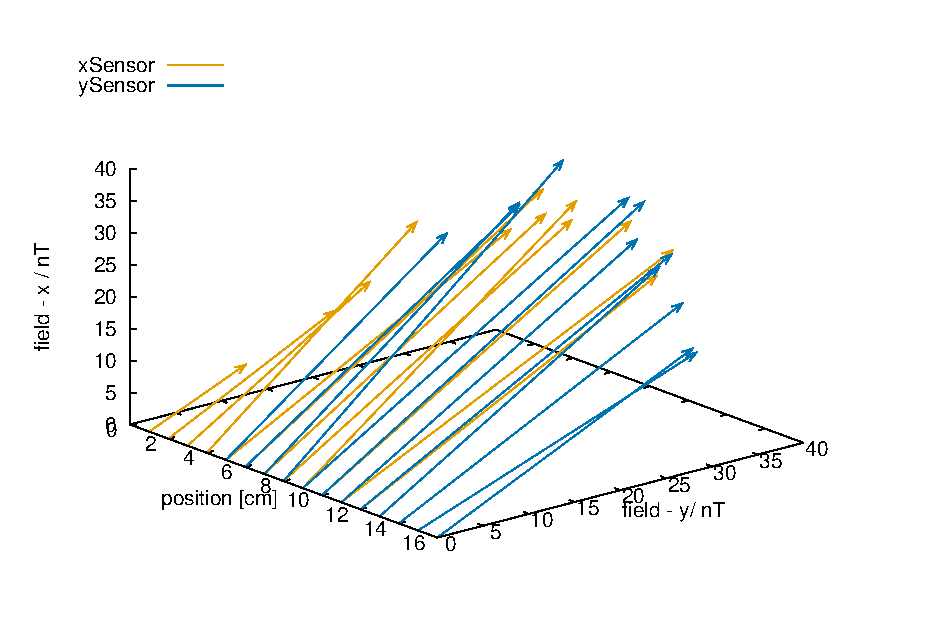
\includegraphics{/home/philipp/Documents/thesis/figures/experiments/fluxgate/spatial3d.eps}
        \end{figure}
\section{Measurements}
    \subsection{Low field NMR}
    Low field spectra were acquired using different setups. The main modification between setups concerned the $B_0$ coil. The initially used solenoid coil showed linewidths of about 0.5 - \SI{1}{\kilo\hertz}. Due to mechanical destruction of one coil and those rather wide lines, a new coil design was simulated and built \ref{simulations:DualHelmholtzArray} using Biot Savart calculations.
    \begin{figure}[h] 
        \centering
        %\includegraphics{}
    \end{figure}
    \begin{figure}[h]
        \centering
        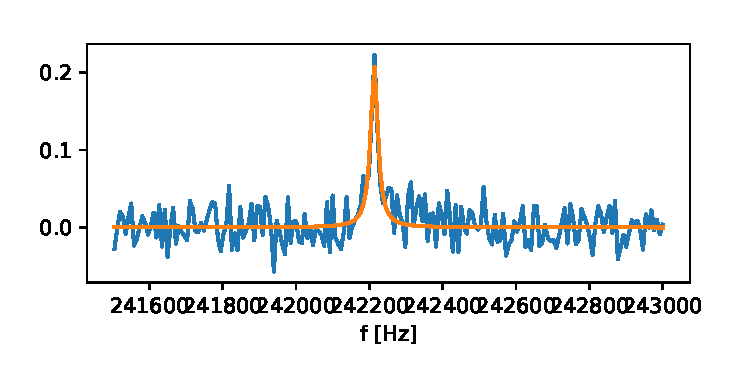
\includegraphics[width = 12cm]{/home/philipp/Documents/thesis/figures/experiments/lowFieldSpectrometer/helmholtzNarrowLine.eps}
    \end{figure}
    \subsection{Sabre in water}
    \begin{figure}[h]
        \subfloat{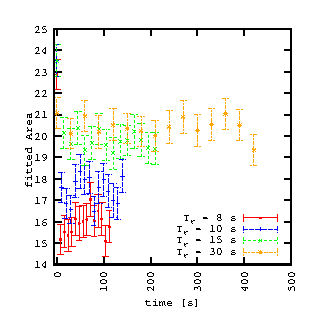
\includegraphics[width = 0.5 \textwidth]{/home/philipp/Documents/thesis/figures/experiments/lowFieldSpectrometer/inSituSabreWater/overlayAll8to30.eps}}
        \subfloat{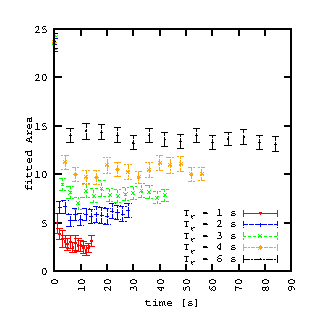
\includegraphics[width = 0.5 \textwidth]{/home/philipp/Documents/thesis/figures/experiments/lowFieldSpectrometer/inSituSabreWater/overlayAll1to6.eps}}
    \end{figure}
    \begin{figure}[h]
        \centering
        \includegraphics[width = 6 cm]{/home/philipp/Documents/thesis/figures/experiments/lowFieldSpectrometer/inSituSabreWater/exponentialFit.eps}
    \end{figure}
    \subsection{Sabre in cell solution and blood}
    \begin{figure}[h]
        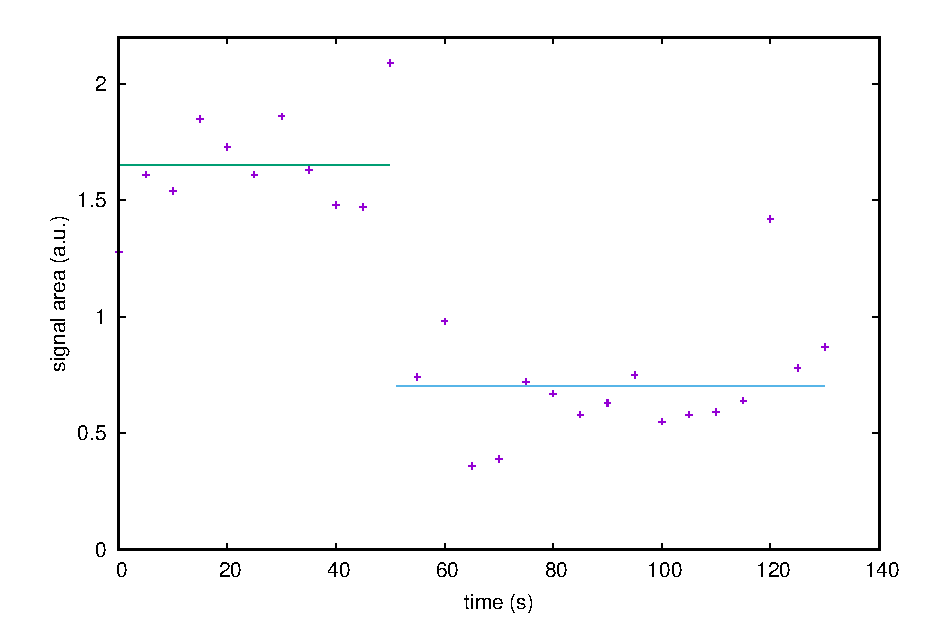
\includegraphics[width=0.9\textwidth]{/home/philipp/Documents/thesis/figures/experiments/lowFieldSpectrometer/inSituSabreWater/cellCultureInjection.eps}
        \caption{Time course of the signal intensity (peak height) when adding human blood to the continuously hyperpolarized solution. Note the string signal drop after addition of \SI{0.5}{\milli\litre} of blood to the solution. The straight and dashed lines indicate the average before and after blood addition.}
        \label{chap:MaterialsAndMethods:bloodInjection}
    \end{figure}
    \begin{figure}[h]
        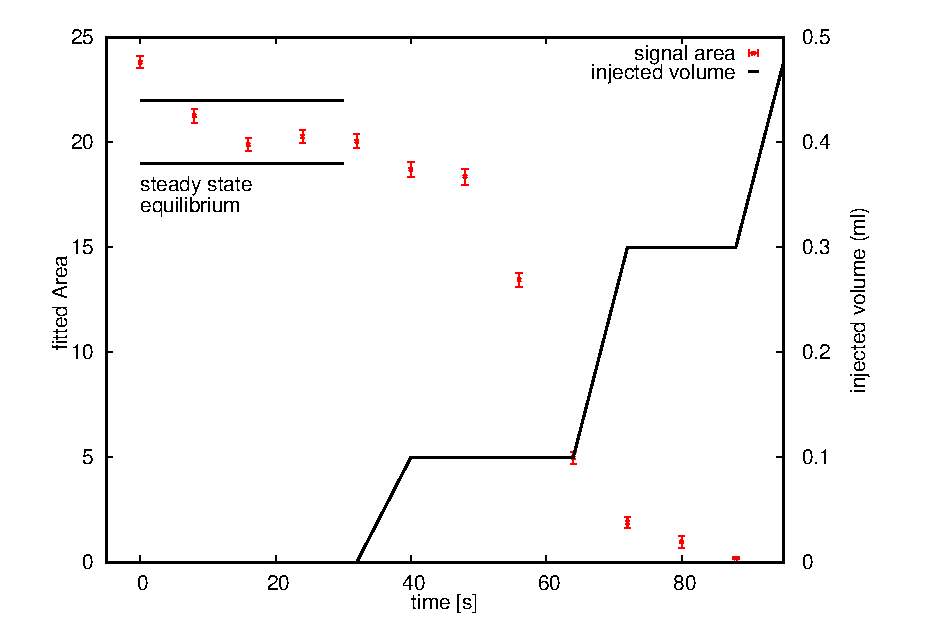
\includegraphics[width=6 in ]{/home/philipp/Documents/thesis/figures/experiments/lowFieldSpectrometer/inSituSabreWater/signalVariation.eps}
        \label{chap:MaterialsAndMethods:bloodInjection2}
        \caption{Signal drop during the injection of \SI{0.5}{\milli\liter} of blood into the solution providing hyperpolarized signal which was permanently provided with fresh pH2.}
    \end{figure}
    \subsection{15N Sabre}
        \subsubsection{15N coil}
        The coil for 15N signal reception was matched and tuned to fit the requiremenst of the system. The network analyzer showed a q-factor of \todo{n} and a width of nn. Inside the small animal NMR, similar resonance widths of nn were observed while the attenuation was \SI{1}{\deci\bel}
    \subsection{Nanotesla field measurements}
        	The field inside the Mu Metal shielding was measured without anny current flowing in the B0 coil as well as with the coil turned on. 
    \subsection{High field Sabre}
\section{Simulations}
        \subsection{Static magnetic field calculations}
            Using the Biot Savart law, a Matlab program to calculate the fields of current carrying conductors was implemented. Structural elements were mostly solenoids, but also saddle and helmholtz coils were considered.
            \subsubsection{solenoid coil}
                The coil used in the low field NMR system was calculated and the length of the compensation windings was optimized for field homogeniety. To do so, the field was calculated inside a $3 x 3 x 3 cm^3$ volume centered inside the coil and plotted as histograms binning fields. An algorithm analyzing over which field 80\% of the fields sampled spread was used as a marker
            \begin{figure}[b]
                \centering
                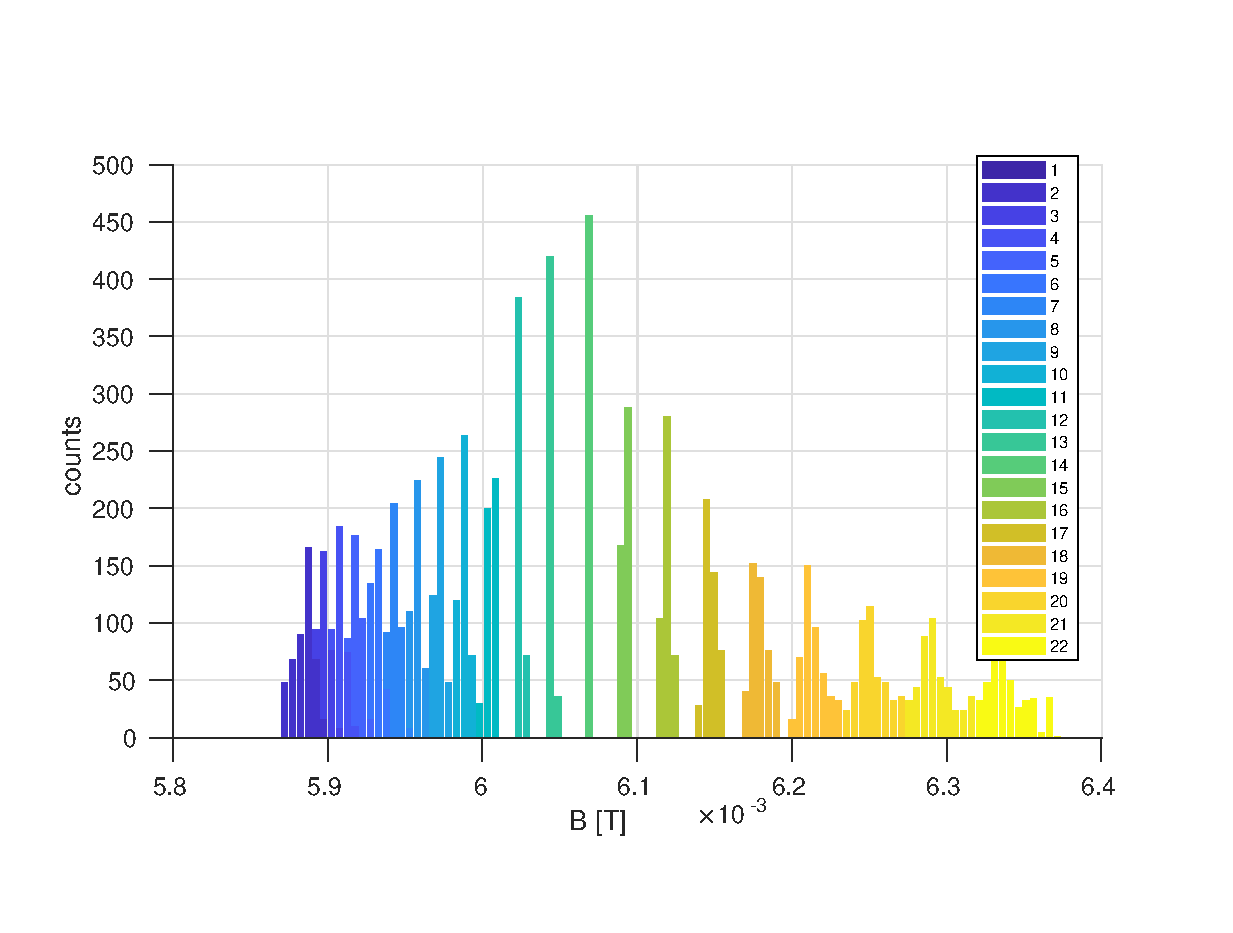
\includegraphics[width=\textwidth]{/home/philipp/Documents/thesis/figures/simulations/B0/solenoidCoil/compensationWinds.eps}
                \caption{Histograms of the magnetic field strength. From left to right, number of compensation windings rise. This leads to a field increase and change in homogeniety.}
            \end{figure}
        \subsubsection{Helmholtz Array}
        The previously used program was also used to simulate the field of the helmholtz array used in later experients. The simulations were used to optimize the parameters for the setup before manufacture. The simulation results concerning the positions of the coils are shown in figure \ref{}. The optimal result is marked, and the field homogeniety is plotted for this result (figure \ref{}). Comparing the field map to figure \ref{} shows a factor \todo{nn} improvement.
        \begin{figure}
            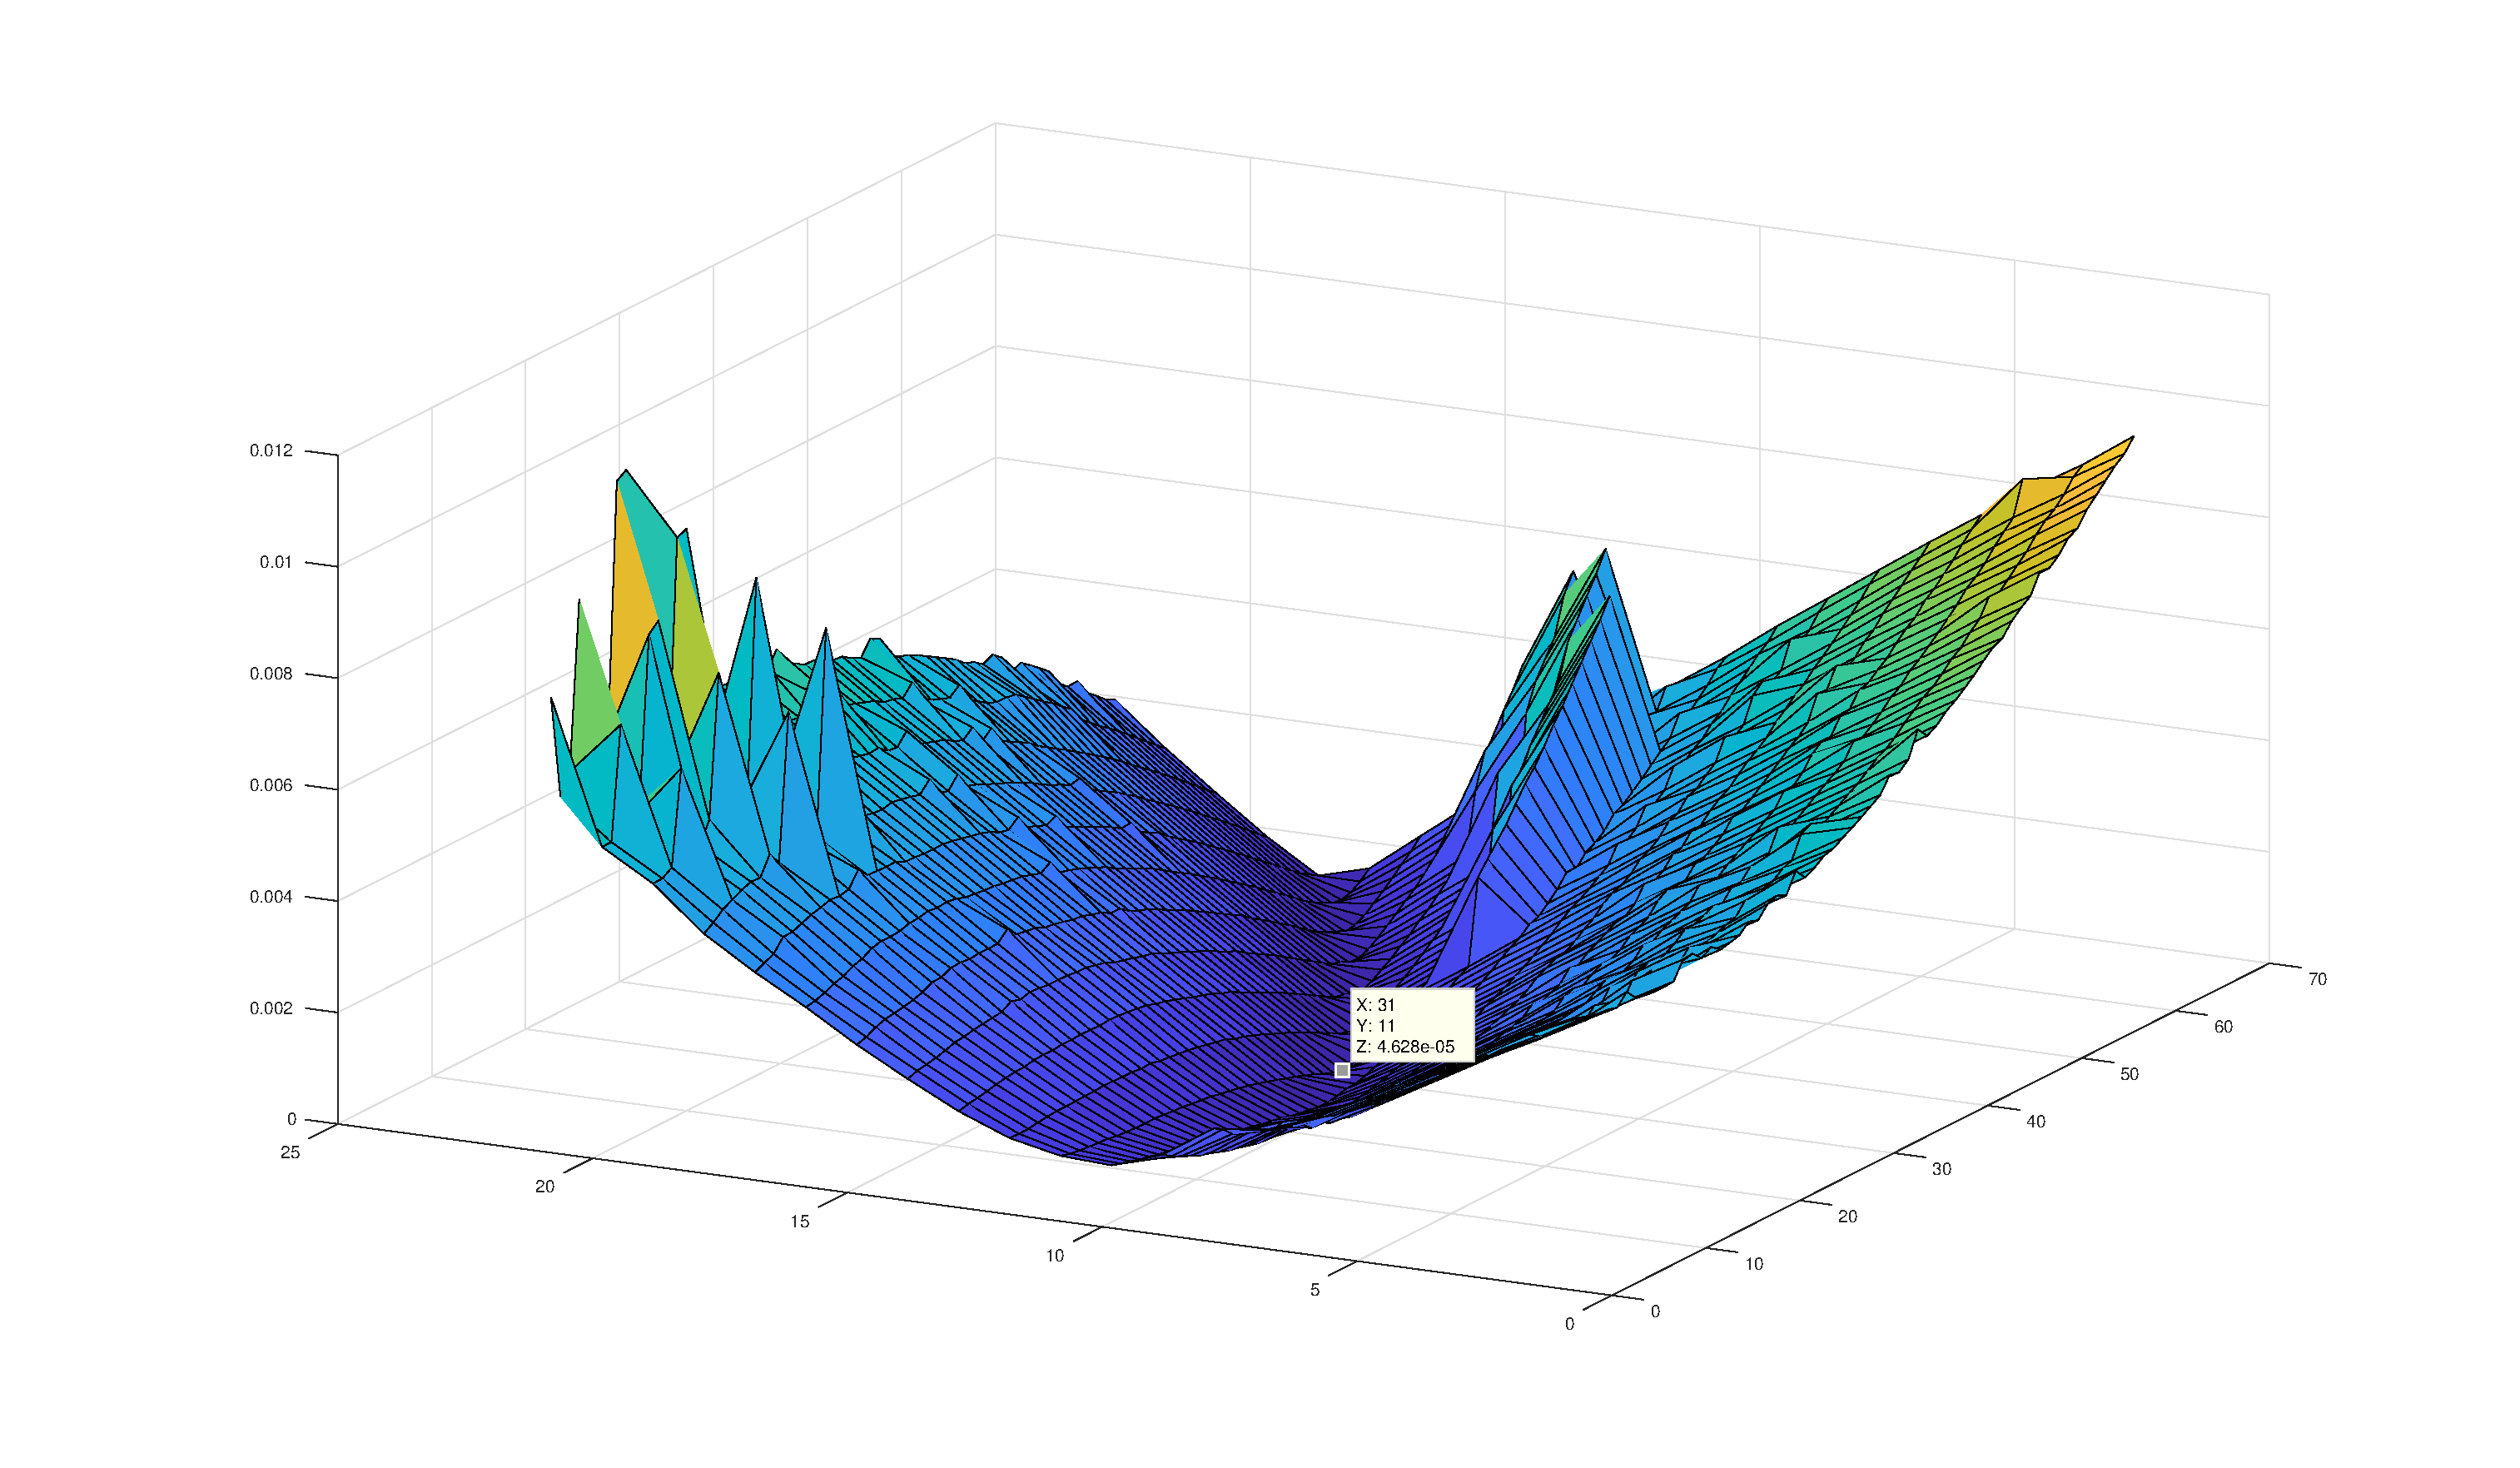
\includegraphics[width = 0.9\textwidth]{/figures/simulations/B0/helmholtzCoil/fieldSpread.eps}
        \end{figure}
%\input{figures/experiments/figExample}
